%%%% ijcai18.tex

\typeout{IJCAI-18 Instructions for Authors}

% These are the instructions for authors for IJCAI-18.
% They are the same as the ones for IJCAI-11 with superficical wording
%   changes only.

\documentclass{article}
\pdfpagewidth=8.5in
\pdfpageheight=11in
% The file ijcai18.sty is the style file for IJCAI-18 (same as ijcai08.sty).
\usepackage{ijcai18}

% Use the postscript times font!
\usepackage{times}
\usepackage{xcolor}
\usepackage{soul}
\usepackage[utf8]{inputenc}
\usepackage[small]{caption}
\usepackage{mathrsfs}
\usepackage{graphicx}
\usepackage[colorinlistoftodos]{todonotes}
\usepackage[colorlinks=true, allcolors=blue]{hyperref}


% the following package is optional:
%\usepackage{latexsym} 

% Following comment is from ijcai97-submit.tex:
% The preparation of these files was supported by Schlumberger Palo Alto
% Research, AT\&T Bell Laboratories, and Morgan Kaufmann Publishers.
% Shirley Jowell, of Morgan Kaufmann Publishers, and Peter F.
% Patel-Schneider, of AT\&T Bell Laboratories collaborated on their
% preparation.

% These instructions can be modified and used in other conferences as long
% as credit to the authors and supporting agencies is retained, this notice
% is not changed, and further modification or reuse is not restricted.
% Neither Shirley Jowell nor Peter F. Patel-Schneider can be listed as
% contacts for providing assistance without their prior permission.

% To use for other conferences, change references to files and the
% conference appropriate and use other authors, contacts, publishers, and
% organizations.
% Also change the deadline and address for returning papers and the length and
% page charge instructions.
% Put where the files are available in the appropriate places.

\title{Poker Project - Team \#36}


% Multiple author syntax (remove the single-author syntax above and the \iffalse ... \fi here)

\author{
Chen Juan, He Zhenfeng, Li Jiawei, Liu Xuan, Tian Xueyan
\\ 
National University of Singapore\\
%
{\{e0253722, he.zhenfeng, li.jiawei, liu.x, tian.xueyan\}}@u.nus.edu\\
}
% If your authors do not fit in the default space, you can increase it 
% by uncommenting the following (adjust the "2.5in" size to make it fit
% properly)
% \setlength\titlebox{2.5in}

\begin{document}

\maketitle

\section{Introduction}
A major topic in modern artificial intelligence is that of building intelligent agents to solve various problems. Extensive-form games comprise a large category of such problems where agents need to make decisions with incomplete and imperfect information given the state of the world. In this project, we explore the procedure of building an intelligent agent playing a typical extensive-form game, a limited two-player version of Texas Hold'em poker. More specifically, we wish to design an agent that can learn from game history and play optimally based on its current knowledge, largely imitating a human player.

A common approach to playing optimally for our agent is to find a Nash equilibrium: playing a strategy that maximizes our utility against the opponent strategy. However, since the information is imperfect in such game, we need to approximate the solutions using estimators. Therefore, we utilize Counterfactual Regret Minimization (CFR) method to calculate regret of the current action and update the strategy. Two versions of online CFR framework are attempted to achieve the best performance. The static estimator version that assumes a static opponent strategy is used during self-training session and obtains strategies that converge to an approximate Nash equilibrium; while the dynamic version, which applies reinforcement learning, is used when playing against unknown agents.

In the implementation process, we evaluate hand-strength of the agent based on Monte Carlo Method and a five-level hand-strength scale. The evaluated hand-strength values in every round are recorded in an overall hand-strength chart, and are used to calculate the winning probability of certain set of hole cards. 

Game history is represented using a 4-base number in the history list, and can be retrieved subsequently by simple arithmetic operation.

After sufficient number of training rounds under the dynamic strategy, we obtain an agent that can achieve a winning rate of 2 dollars per iteration against a raising agent, which is equivalent to 0.2 small-bets-amount.

\section{Related Work}

This section introduces basic strategy concept and notations, as well as the definition and representation of Nash Equilibrium, which helps explaining algorithm design and implementation consideration. 

\subsection{Strategy}

Given an information set $I_i$ and an action set $A(I_i)$, we define the strategy of a player $i \in N$ as $\sigma_i$, where $N$ is the set of all the players in the game. $\sigma_i$ is a probability distribution function about $A(I_i)$, $\sigma_i$($I_i$):$A$($I_i$) $\rightarrow$ [0,1].\\
A strategy profile should consist of all the strategies of every player in the game, therefore $\sigma$ = ($\sigma_1$, $\sigma_2$, ... , $\sigma_{|N|}$). We use $\sigma_{-i}$ to denote all the strategies except $\sigma_i$, $\sigma_{-i}$ = $\sigma$ / {$\sigma_i$}.

\subsection{Nash Equilibrium}

\subsubsection{Best Response}

We define history $h$ as a set of action sequences. With a given strategy profile $\sigma$, the history $h$ has a happening probability $\pi^{\sigma}(h)$.  A player $i$ has an expected utility value
$\mu_i(\sigma) = \sum_{h \in Z} \mu_i(h) \pi^{\sigma}(h)$, given $\sigma$ and $h$, where $Z$ is the set of terminal history.

The player $i$ has an optimal response strategy $\sigma_i^*$ based on $\sigma_{-i}$, that satisfies $\mu_i$($\sigma_i^*$, $\sigma_{-i}$) $\geq$ $\max_{\sigma_i^{\prime} \in \sum_i}$ $\mu_i$ ($\sigma_i^\prime$, $\sigma_{-i}$). In a strategy profile $\sigma$, if every player's strategy is the best response in other players' strategy profile, then $\sigma$ is a Nash Equilibrium strategy.

\subsubsection{Nash Equilibrium}

A strategy profile $\sigma$ = ($\sigma_1^*$, $\sigma_2^*$,...,$\sigma_{|N|}^*$) is a Nash Equilibrium strategy if and only if for each player $i \in N$, the player has $\mu_i$($\sigma$) $\geq$ $\max_{\sigma_i^\prime \in \sum_i}$ $\mu_i$ ($\sigma_1^*$,$\sigma_2^*$,...,$\sigma_i^\prime$,...,$\sigma_{|N|}^*$). We define that $\sigma_i^\prime$ is any other strategy of player i except $\sigma_i^*$.

\subsubsection{$\varepsilon$-Nash Equilibrium}

An approximation of Nash Equilibrium is called $\varepsilon$-Nash Equilibrium. For a given positive real number, strategy profile $\sigma$ is a $\varepsilon$-Nash Equilibrium if and only if for every player $i \in N$, it has 
$\mu_i(\sigma) + \varepsilon \geq \max_{\sigma_i^\prime \in \sum_i} \mu_i(\sigma_i^\prime, \sigma_{-i})$. 
If this game is played for sufficiently large number of times $t$, we define that the strategy profile as $\sigma^t$. If the game has been done $M$ times, then in these $M$ games, for a player $i \in N$, the average overall regret is defined as 

$R_i^m = \frac{1}{M} \max_{\sigma_i^* \in \sum_i}
\sum_{t=1}^M (\mu_i(\sigma_i^*, \sigma_{-i}^t) - \mu_i$($\sigma^t))$.

Especially in this game, only 2 players, at time $t$, if both of the two players have an average overall regret value less than $\varepsilon$, then the average value of the 2 players' strategy profile, $\sigma^{-t}$, is 2$\varepsilon$-Nash Equilibrium strategy.

\section{Method}

This section explains the framework we used to approximate Nash Equilibrium and update strategies in the design and implementation of our agent.

\subsection{Counterfactual Regret Minimization}

In order to approach Nash Equilibrium in this game with imperfect information, we apply the method of Counterfactual Regret Minimization. This method iterates through all information sets; during which an information set is visited, counterfactual value (CF value) and counterfactual regret (CF regret) are computed.

\subsubsection{Counterfactual Regret}

For player $i$ and information set $I \in \mathscr{I}$, the CF value of $I$ about the strategy set $\sigma^t$ is defined as

$v_i(\sigma^t, I) = \sum_{z \in Z_I} u_i(z) \pi_{-i}^{\sigma^t}(z[I]) \pi^{\sigma^t}(z[I], z)$,\\
where $Z_I$ is the set of all the terminal states that passes $I$, and $z[I]$ is the prefix of terminal state $z$ in $I$.

In fact, only the computation of the CF values in terminal information sets requires the above equation. For a non-terminal information set $I$, its CF value can be computed by

$v_i(\sigma, I) = \sum_{I' \in Succ(I)} v_i(\sigma, I') \pi_i^\sigma(I, I')$,
\\where $Succ(I)$ is the set of the successive information sets of $I$, and $\pi_i^\sigma(I, I')$ is the transition probability from $I$ to $I'$.

For player $i$ and information set $I \in \mathscr{I}$, the CF regret of every action $a \in A(I)$ on $I$ at time $t$ is defined as

$r_i^t(I, a) = v_i(\sigma_{I \rightarrow a}^t, I) - v_i(\sigma^t, I)$\\
where $\sigma_{I \rightarrow a}^t$ is almost the same strategy set as $\sigma^t$, but on information set $I$ it will always choose action $a$. It denotes the difference between CF values of executing action $a$ and action decided by $\sigma^t$. If the value is positive, the agent should execute more of action $a$, otherwise there will be more regrets.

The CF regrets of every information set after each iteration will be used to calculate the game strategies for the next round of iteration. The new strategy are be generated by regret matching\footnote{$\sigma(I_i,a)=\frac{R_i(I_i,a)-MinR}{\sum_{a'\in A(I_i)}R_i(I_i,a')-MinR}$, where $MinR = Min(R_i(I_i,a'), a'\in A(I_i))$}. By updating strategies through these iterations , we are able to minimize the average regret for the agent, thus approaching Nash Equilibrium.

\subsubsection{Online CFR Minimization Framework}

\noindent\textbf{Step 1. Initialization}

For each of the information set $I_i \in \mathscr{I}_i$, we initialize its CF value as $v_i(I_i) = 0$; for every possible action $a \in A(I_i)$ on $I_i$, its CF regret as $r_i(I_i, a) = 0$, its execution probability as $\sigma_i(I_i, a) = \frac {1} {|A(I_i)|}$.\\
\noindent\textbf{Step 2. Repetitions of the Game}

For each round of the game:

\begin{enumerate}
\item Play with the opponent according to strategy $\sigma_i$;
\item Record the result of the game $u_i$ and pass it to the CF value calculator;
\item For every information $I_i$ set visited during this round of the game, obtain its estimated CF value through the calculator.
\item For every information $I_i$ set visited, update its CF regret $r_i$ and strategy $\sigma_i$.
\end{enumerate}

For each round of the game, the player plays the game according to the current strategy $\sigma_i$, and obtains the game result, which is passed to the CF value calculator to generate the CF value. Then the CF regrets and relative strategies are updated for future games.

In real game situations, as the opponent's strategy is unknown, it is usually impossible to directly calculate the actual CR values. However, we can use estimated CR values to approximate the minimized CF regrets with a certain probability. Thus we replace the ``CF value calculator" which  generates the actual CF values with the ``CF value estimator" which generates the estimations of CF values in the above steps.

Based on these facts, algorithms are proposed to complete the estimations. Two different types of implementations of the estimators of CF values are illuminated below.

\subsection{Static Estimator}

Static estimator assumes that the opponent has a static strategy to play the game, thus, we can learn and compute the approximate regret value from the sample of the game result.

As the CF values of the non-terminal information sets can be deduced by those of the terminal information sets, only the estimation of CF values of the terminal information sets is necessary.

\subsubsection{seOCFR Algorithm}

Online CFR minimization algorithm based on the method of static estimation.

\textbf{Input}: Current number of rounds of games $M$, the cumulative result on each of the terminal information set $S_i$, the CF values of each of the terminal information set $V_i$, and the CF regrets $R_i$.

\textbf{Output}: $V_i$, $R_i$, $\sigma_i$

\textbf{Step 1}: Play a round of game, and for each action of the round,
\begin{enumerate}
\item Make the decision according to current strategy $\sigma_i$;
\item If some terminal information set $I_z$ is visited, obtain the game result $u_i$, $S_i(I_z) = S_i(I_z) + u_i$; let $\pi_i^\sigma$ be the contribution of $\sigma_i$ to reach $I_z$, $V_i(I_z) = \frac {S_i(I_z)} {\pi_i^\sigma M}$
\end{enumerate}

\textbf{Step 2}: Let $I_i$ be an information set visited before $I_z$ is visited,

\begin{enumerate}
\item $V_i(\sigma, I) = \sum_{I' \in Succ(I)} V_i(\sigma, I') \pi_i^\sigma(I, I')$;
\item If $P(I_i)$ equals $i$,

for every action $a \in A(I_i)$, $R_i(I_i, a) = R_i(I_i, a) + V_i(I a) - V_i(I)$.

$\sigma_i(I_i) = regretMatching(I_i)$.
\end{enumerate}

\textbf{Step 3}: Repeat Step 2 until $I_i$ is empty.

\subsection{Dynamic Estimator}

In the static estimator, it assumes that the opponent strategy remains the static, then, the game result distribution will be determined only by the two players' strategy. The static estimator is to give each game result an equal height, $\frac {1} {M(I_r)}$. However, if the opponent consistently changes his strategy, which is highly possible, the game result distribution will change consistently and accordingly. Hence, to estimate a more accurate regret value, we introduce the dynamic estimator.

\subsubsection{Reinforcement Learning}

The dynamic estimator can be regarded as an application of reinforcement learning. Agents learn by getting rewards from interacting with the environment in reinforcement learning. It is a process of evaluation and feedback. If an agent takes some action or strategy, the environment changes with the action accordingly and produces a reward as feedback to the agent. The agent chooses the next action based on the feedback from the environment and the state of the environment. If the agent receives a positive reward from the environment, in the future, it is more likely for this agent to take the same action or strategy. The agent is to find the optimal strategy to maximize the sum of the expected rewards. In reinforcement learning, the agent learns by its own experience and rewards, instead of what the environment tells what agent should do.

\subsubsection{deOCFR Algorithm}

Online CFR minimization algorithm based on the method of dynamic estimation.

\textbf{Input}: Learning rate $\alpha_1$ ($ 0 < \alpha_1 < 1$) and $\alpha_2$ ( 0 < $\alpha_2 < 1$), table Q to store action utility value of each information set, table $\nu_i$ to store the CF value of each information set, table $R_i$ to store CF regret value of each information set. 

\textbf{Output}: $V_i$, $R_i$, $\sigma_i$

\textbf{Step 1}: Initialization of each value in table Q;

\textbf{Step 2}: Let $I_i$ be the information set when the first strategy needed for player $i$ in the game;

\textbf{Step 3}: Choose an action a based on I and selected strategy $\sigma_i$;

\textbf{Step 4}: For every actions afterwards in the game:

\begin{enumerate}
\item Let $I_i'$ be the information set needed for decision or the terminal information set after $I_i$;
\item Inspect the reward $r$ from $I_i$ to $I_i'$;
\item Based on strategy $\sigma_i$, choose an action $a'$ on $I_i'$;
\item $Q(I_i, a) = \alpha_1 Q(I_i, a) + \alpha_2 (r + Q(I_i', a'))$;
\item $V_i(I_i) = \sum_{a \in A(I_i)} Q(I_i, a)$;
\item Let $\pi_i^\sigma$ be the contribution of $\sigma_i$ to reach $I_i$;
\item For each $a \in A(I_i)$,

$R_i(I_i, a) = R_i(I_i, a) + \frac {Q(I_i, a) - V_i(I_i)} {\pi_i^\sigma}$;
\item $\sigma_i(I_i) = regretMatching(I_i)$;
\item $I_i = I_i'$, $a = a'$.
\end{enumerate}

\section{Application}
This section describes implementation details of the agent.
\subsection{Abstraction}

We want to build a metric to evaluate the winning probability during the game process for every betting round. Using only Monte Carlo Method to calculate the hand-strength is not comprehensive enough since there are only four rounds in total. This abstraction intended to withdraw five evenly divided point of probabilities in order to classify the hand-strength in each round by level 1-5.

\subsubsection{Hand-strength Evaluation}


At the beginning of every round, each player holds two hole cards with no knowledge of the community cards. With the only knowledge of two hole cards in hand, the way to evaluate the winning probability is using Monte Carlo Method. We first randomly generating the left 5 community cards and the opponent’s two hole cards from unused cards. Using each of the randomly generated cards, we can decided who is the winner by evaluating the hand strength using the existing method which is intuitive. Repeatedly record the winner every time and calculate the player’s number of winning round among 1000 times of random generation\footnote{By Bernoulli experiment, the result has 3\% errors under 95\% confidence interval}. Suppose the number of winning round is $x$, then we can get a winning probability of $\frac{x}{1000}$ of our hole cards.

\subsubsection{Overall Hand-strength Chart}

After calculating the probability of winning at pre-flop betting round for every possible combination of two hole cards, we can sort the probability in ascending order and evenly divide them into 5 parts using 4 quarter-point. Thus, we can classify the hole card as one of the hand-strength as [1, 2, 3, 4, 5] level by allocating its winning probability in one of the 5 parts. 
At the flop betting round, players have a knowledge of the 3 community cards. Similarly using the Monte Carlo Method to randomly generate the left two community cards and opponents hole cards to calculate the winning probability. In the same way as pre-flop round, this will generate five levels using 4 quarter-point of winning probability\cite{carmelo}.

Doing the same procedure to next two betting rounds, this method will output totally four winning probability for every hole cards in a game round, representing the winning probabilities of the hole cards in pre-flop, flop, turn and river rounds as [p(pre-flop), p(flop), p(turn), p(river)].

In the end of this procedure, a probability chart will be generated representing the winning probability of a hole card as $[p1, p2, p3, p4]$ if its hand-strength in each round is $x1, x2 ,x3 ,x4 (1\leq xi\leq5)$.

Transform this probability array into a numerical value representing the approximated overall winning rate as ($p1\times6^3 + p2\times6^2 + p3\times6^1 + p4$).


\subsubsection{History Representation}

As for the representation of the history of game, we record big-blind as 1 and otherwise as 0 at the very beginning of each round. In every betting rounds pre-flop, flop, turn and river, we represent raise as 1, call as 2, fold as 3. Following the above encoding method, we can record the game history use a 4-base number in the history list. For example, a encoding can be $(xabcd)_4$  
\footnote{This encodes a round with four actions, where $x$ is either 0 or 1, representing whether the agent is big-blind; $abcd$ represents four actions (raise, call or fold) in the sequence. Hence the encoding value is calculated as $x\times4^4+ a\times4^3 + b \times 4^2+ c\times4^1+d\times4^0 $}.
Thus we can use modulo operation to trace back the previous action we made.

\subsection{Training, Improvement, Tournament}

With the abstracted information set, we can use counterfactual regret minimization to compute an approximate equilibrium algorithms for this game. To train our agent, we decide to use self-training and seOCFR algorithm. With sufficient training, the strategies will converge to an approximate Nash equilibrium. In this training, as both agents use static strategies, the counterfactual value computed by seOCFR has higher convergence rate,therefore seOCFR will have better performance than deOCFR.

Extending to working with the Limited Texas Hold’em, we did some modifications on the original seOCFR procedure. For example, instead of initializing every counterfactual value $v_i$($\sigma$,$I$)= 0, we pre-compute the payoff of each $fold$ action, and initialize the counterfactual value as the payoff, as the value of every terminal information set ends with $fold$ action is certain. We also set the $\sigma_i$($I$, $fold$) = 0 by default. The reason of doing this is that to increase the speed of the training such that the agent does not need to traverse the $fold$ action to get its counterfactual value.

When playing against another unknown agent, we use the pre-trained result from the self-training and deOCFR algorithm. The pre-trained result can prevent our agent from losing money at the initial several rounds. Using deOCFR algorithm can help our agent to learn the opponent agent quickly as deOCFR algorithm puts more weights on the latest learning results. We could also improve on the opponent model to 

\section{Experiment}


\begin{figure}[hbt!]
\centering
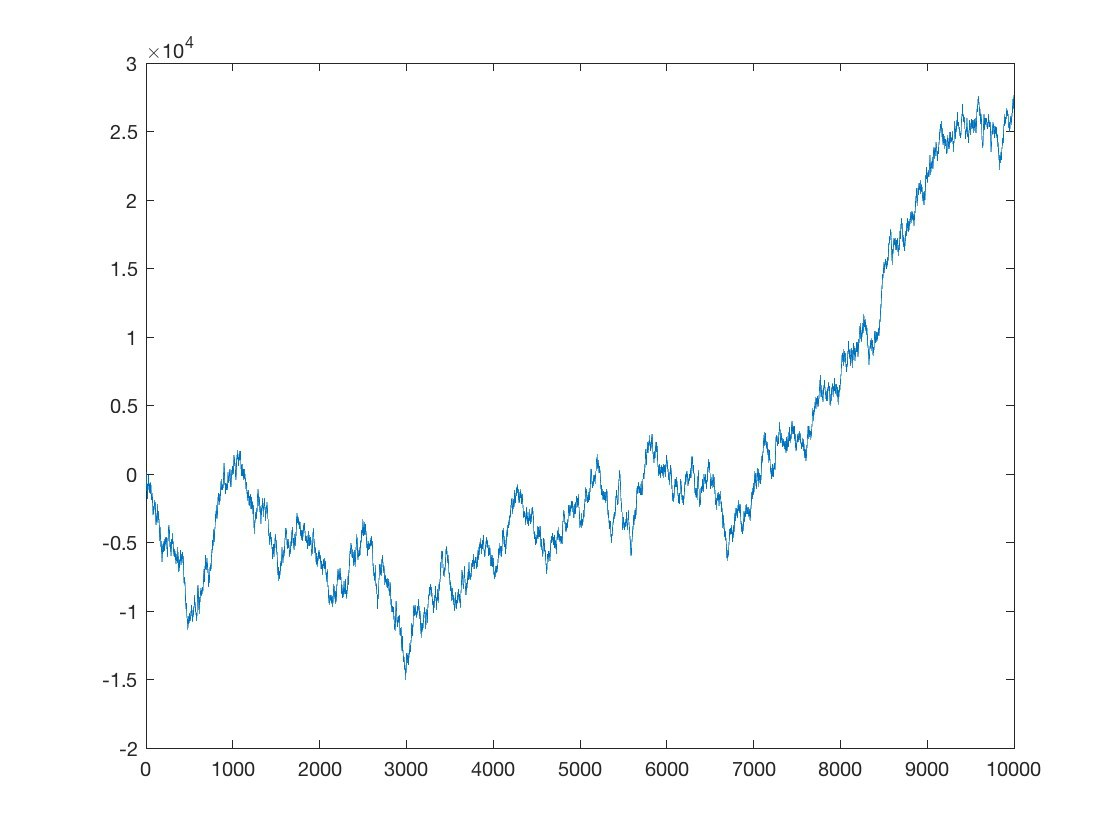
\includegraphics[scale=0.1]{win.jpg}
\caption{\label{fig:win}Winning-rate against a raising agent}
\end{figure}

\begin{figure}[hbt!]
\centering
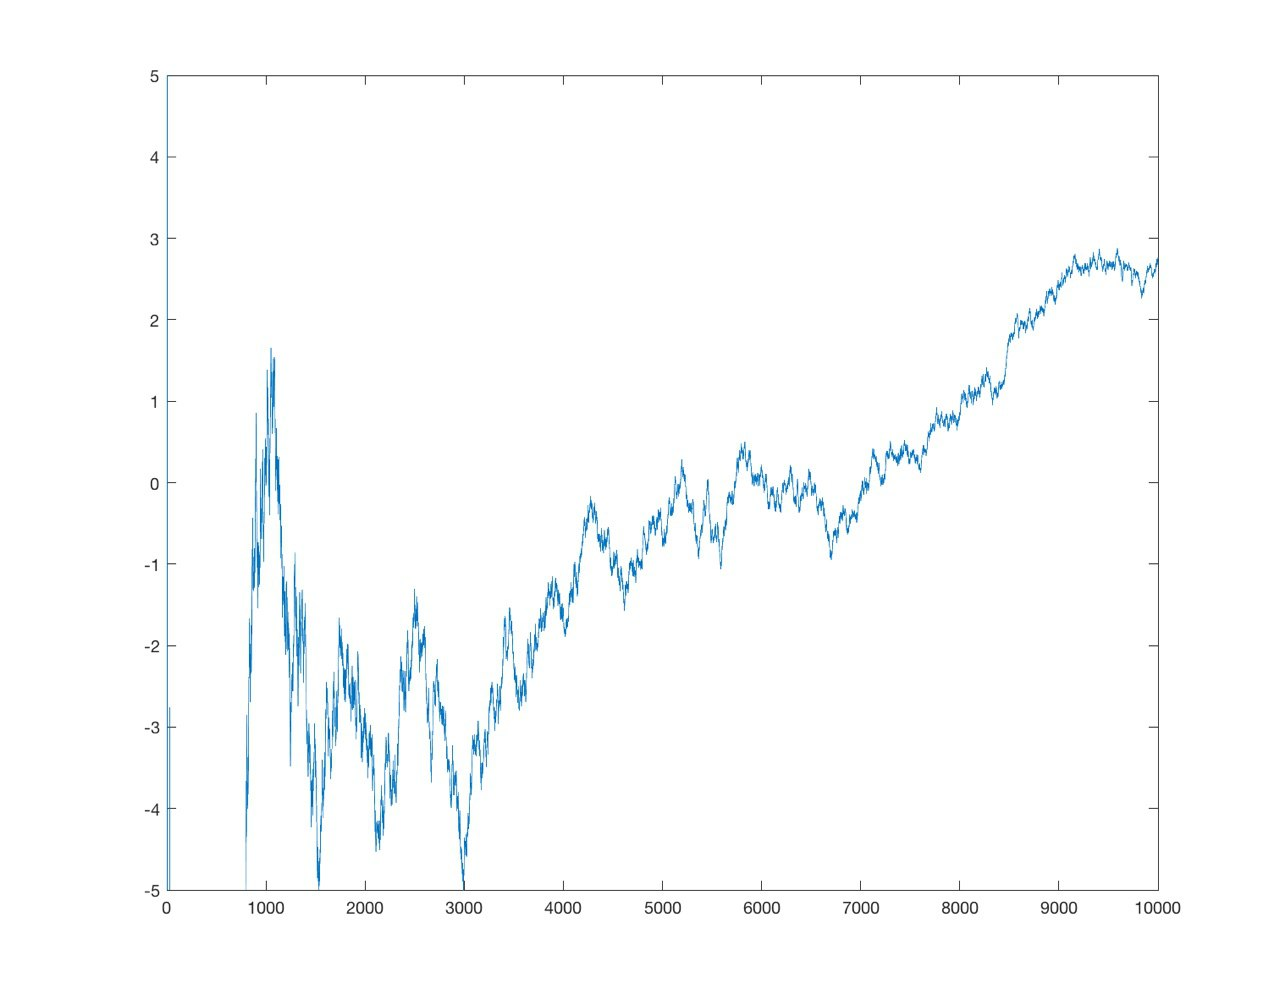
\includegraphics[scale=0.1]{average.jpg}
\caption{\label{fig:average}Average winning-rate against a raising agent}
\end{figure}

\begin{figure}[hbt!]
\centering
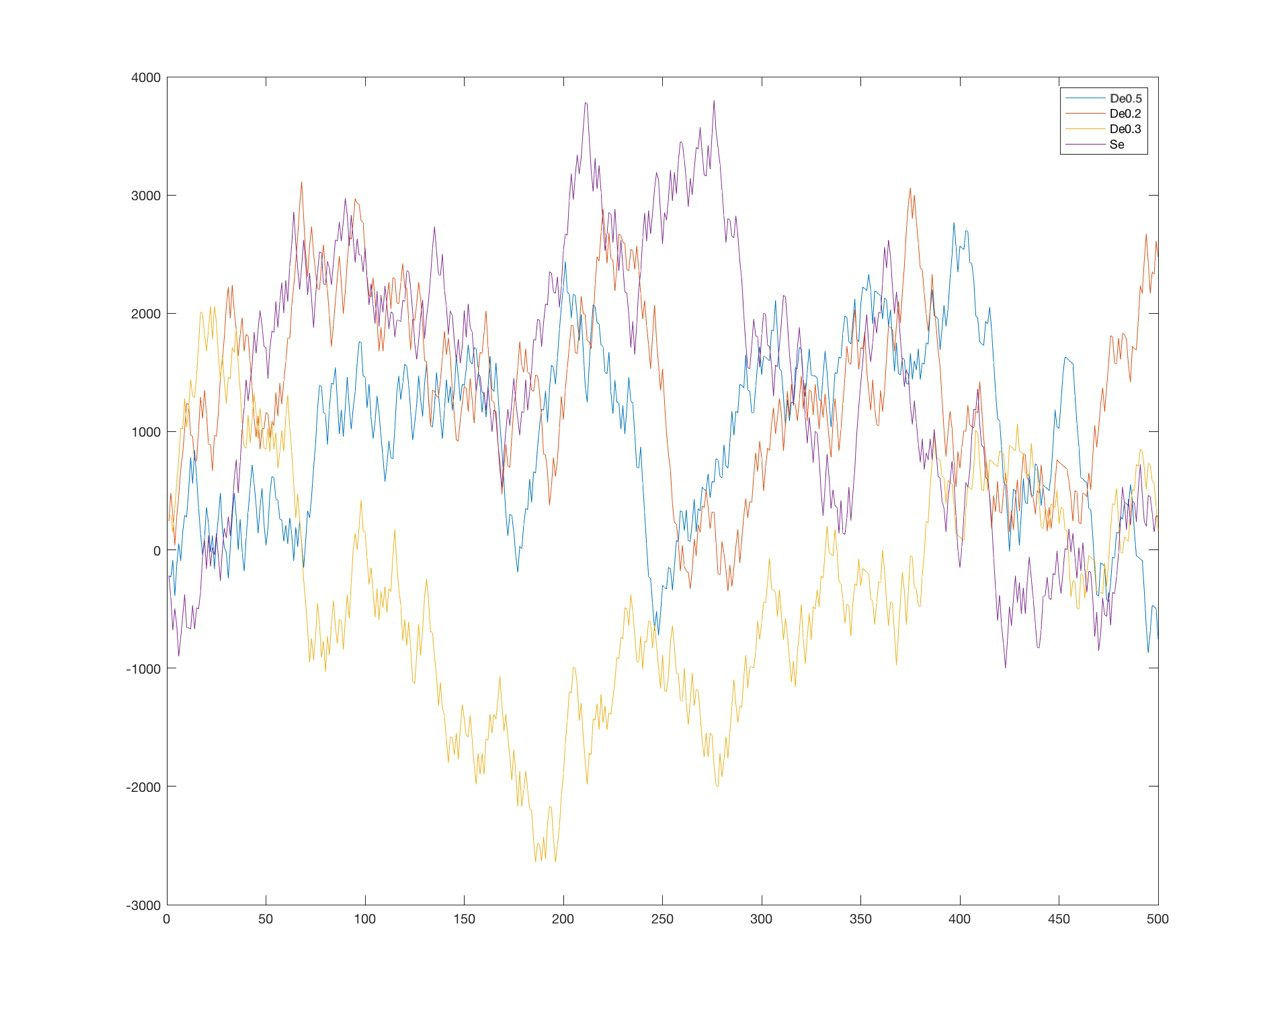
\includegraphics[scale=0.12]{500games.jpg}
\caption{\label{fig:500games}Performance of different algos against a raising agent}
\end{figure}
This section presents the results of our agent playing against a raising agent\footnote{A raising agent is an agent always raises if possible, and never folds}. Figure \ref{fig:win} and Figure \ref{fig:average} shows the performance over 10000 iterations without pre-training. Figure \ref{fig:500games} shows the performance of different algorithms against a raising agent over 500 iterations with pre-training.

Figure \ref{fig:win} shows the winning amount. It indicates that our agent performs weakly at the beginning, but with sufficient training\footnote{In this experiment, there is an increasing trend since around 7000 iterations}, our agent has significantly improved on the performance. Figure \ref{fig:average} is the average winning amount\footnote{Average winning amount = total winning amount / number of iterations} plot. It indicates that after sufficient training, our agent can achieve a winning rate of 2 dollars per iteration , which is also 0.2 small-bets-amount/iteration.  

Figure \ref{fig:500games} shows the performance of seOCFR and deOCFR with different weights. We found that giving 0.2 weight for the latest result has best performance in this experiment.

\section{Conclusion}
Overall, we are able to achieve an encouraging results using our agent to get a winning rate of 2 dollars per iteration.

In the future, there is definitely potential to improve the agent. First of all, the training time should be extended to ensure that every information set and terminal state can be visited sufficient times\footnote{We would assume $10^9$ times to guarantee the agent is sufficiently trained}. We could also build more opponent models other than simple raising, random and self-training to simulate real-world Texas Hold'em game play. 

Further exploration of algorithm architectures could potentially improve our results as well. We can divide hand-strength into 10 partitions to obtain a more accurate model. Other reinforcement learning algorithms such as Q-learning could be attempted alternatively to obtain a better strategy training.





\appendix

\section{Acknowledgments}

We thank Dr. Yair Zick \texttt{dcsyaz@nus.edu.sg} and Mr. Arka Maity \texttt{e0146321@u.nus.edu} from CS3243 teaching staff team for their supervisions and help with this project.
 
\bibliographystyle{named}
\bibliography{ijcai18}
 
\end{document}
